   \documentclass{article} % Change to a standard article class
   \usepackage{amsmath} % for math environments and commands
   \usepackage{cite}
   \usepackage{amssymb}
   \usepackage{amsfonts}
   \usepackage{graphicx}
   \usepackage{textcomp}
   \usepackage{xcolor}
   \usepackage{subcaption} % Adicione isso no preâmbulo do seu documento
   \usepackage{float} % For [H] placement option



   \begin{document}

   \title{KNN ponderado e SVM na predição de Câncer de mama.\\
   }

   \author{Arthur Felipe Reis Souza \\
   Electrical Engineering Department, \\
   Federal University of Minas Gerais, \\
   Belo Horizonte, Brazil \\
   arthurfreisouza@gmail.com \\
   \and
   Antônio de Pádua Braga and Frederico Gualberto Ferreira Coelho \\
   Electrical Engineering Department, \\
   Federal University of Minas Gerais, \\
   Belo Horizonte, Brazil \\
   apbraga@cpdee.ufmg.br, fredgfc@ufmg.br
   }

   \maketitle

   \begin{abstract}
      % Abstract content here.
   \end{abstract}

   \section{Introdução}

   O câncer de mama é uma condição que se caracteriza pelo crescimento descontrolado de células malignas no tecido mamário, afetando tanto homens quanto mulheres, embora seja mais prevalente entre as mulheres. Os riscos para o desenvolvimento desse tumor aumentam com a idade, histórico familiar de casos anteriores e hábitos de vida, como obesidade, sedentarismo, e vícios em álcool e tabaco. Os principais sintomas incluem alterações no formato da mama, inchaço e irritação, dor nos seios e a presença de um nódulo na região mamária. Este relatório tem como objetivo, com base em um conjunto de dados de 568 pacientes, prever se o tumor é maligno ou benigno. Para essa predição, foram utilizados dois algoritmos: KNN ponderado e Máquina de Vetor de Suporte (SVM). Os hiperparâmetros de ambos os modelos foram ajustados para compreender seu desempenho, e a seleção dos parâmetros finais foi realizada por meio do algoritmo de GridSearch Cross-Validation.

   \vspace{1cm}

   As características que resultam em um rótulo são extraídas por meio de uma análise matemática das mamografias (raios X da região mamária), onde esses elementos representam distâncias nas imagens. Esses valores matemáticos são cruciais para a predição, pois alimentam o classificador, que determinará se o tumor é maligno ou benigno.

   \vspace{1cm}

   \begin{figure}[h] % 'h' posiciona a figura aproximadamente no local do código
      \centering % centraliza a figura
      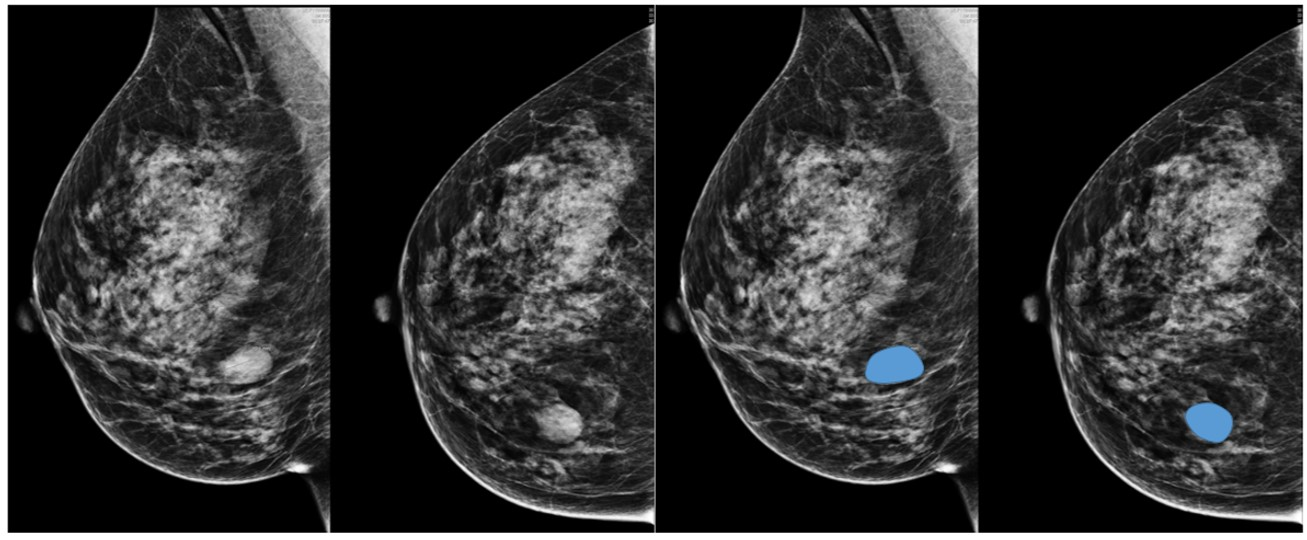
\includegraphics[width=0.75\linewidth]{mamografia.jpg} % insira o caminho da sua imagem e ajuste a largura
      \caption{Foto resultante de uma mamografia.} % insira a legenda desejada
      \label{fig:exemplo} % rótulo para referenciar a figura no texto
   \end{figure}

   \vspace{1cm}

   Apesar de ser um problema mais comum entre mulheres, o câncer de mama também ocorre em homens, muitas vezes de maneira mais nociva, devido ao fato de que o tumor é frequentemente descoberto em estágio avançado de metástase. Além disso, a estrutura mamária dos homens é menor e está mais próxima do peito. Quando o câncer é diagnosticado, o paciente geralmente precisa passar por um tratamento mais agressivo, o que, em muitos casos, pode levar tragicamente à morte.

   Com o desenvolvimento tecnológico, a utilização de algoritmos de aprendizado de máquina se torna uma ferramenta importante para a análise de padrões e a detecção de doenças. O algoritmo mais comumente utilizado na análise de imagens é o das Redes Neurais Convolucionais, que aplicam uma série de filtros na imagem principal para extrair o máximo de detalhes possíveis, ajudando o classificador final a tomar uma decisão. No entanto, neste exercício, elas não serão utilizadas, pois o objetivo é mostrar o desempenho do KNN e da SVM ao variar seus hiperparâmetros.

   \section{Desenvolvimento}

   A base de dados contém 568 linhas e 31 colunas, sendo uma delas a coluna de rótulos. A predição do classificador indica que um rótulo de 1 resulta em um tumor maligno, enquanto -1 indica um tumor benigno. Inicialmente, os rótulos e as características foram separados. Após essa separação, foi realizada a normalização dos dados. Primeiramente, utilizou-se o StandardScaler, cuja fórmula é dada por 

   \[
   z = \frac{x - \mu}{\sigma}
   \]

   Em seguida, aplicou-se o MinMaxScaler, que é representado pela equação 

   \[
   x' = \frac{x - x_{\text{min}}}{x_{\text{max}} - x_{\text{min}}}
   \].

   \vspace{1cm}

   Após a normalização dos dados, estes foram divididos em conjuntos de treino e teste, com 70\% dos dados destinados ao treino e 30\% ao teste. Cada um dos algoritmos teve seus hiperparâmetros ajustados por meio de uma busca em grade (Grid Search). Para a SVM, o hiperparâmetro \( C \) variou de 0.01 até 2, com um incremento de 0.01. Foram testados quatro diferentes kernels: 

   1. Kernel Linear:
      \[
      K(x, y) = x^T y
      \]

   2. Kernel Polinomial:
      \[
      K(x, y) = (\alpha x^T y + c)^d
      \]

   3. Kernel RBF (Gaussiano):
      \[
      K(x, y) = e^{-\frac{\|x - y\|^2}{2\sigma^2}}
      \]

   4. Kernel Sigmoidal:
      \[
      K(x, y) = \tanh(\alpha x^T y + c)
      \]

   Para o KNN, o valor de \( K \) foi variado em um Grid de 1 até 50, enquanto o hiperparâmetro \( h \), que controla a abertura da Gaussiana, foi ajustado manualmente.

   % Data Generation content here.

   \section{Resultados e Discussão}

   \subsection{SVM}

   \vspace{1cm}

   Após a aplicação do Grid Search na SVM, os melhores hiperparâmetros identificados foram \(C = 1.5\), combinados com um kernel linear e normalização Z-Score, resultando em um tempo de execução de 27 segundos e uma acurácia de 98\%. Ao optar pela normalização MinMax, os hiperparâmetros ajustados foram \(C = 1.2\), também com kernel linear, mantendo uma acurácia de 98\% e com um tempo de treinamento de 35 segundos. Esse padrão perdurou por várias vezes em que o código foi executado. Um ponto interessante a destacar é que, sem normalização, o tempo de Grid Search aumentou significativamente, atingindo 2000 segundos. Nesse caso, os hiperparâmetros utilizados foram \(C = 1.84\) com kernel linear, resultando em uma acurácia de 95\%. Isso evidencia que a ausência de normalização faz com que o modelo SVM leve muito mais tempo para ser treinado.

   \vspace{1cm}

   A escolha do kernel linear pelo método GridSearch indica que a base de dados possui características lineares. Definir o kernel ideal para o classificador SVM exerce influência direta na precisão da classificação final, alterando significativamente o padrão da superfície de separação. O método mais comum para selecionar o tipo de kernel é o algoritmo GridSearch, que testa cada kernel combinado com diferentes valores de hiperparâmetro C, com o objetivo de encontrar a melhor combinação de acordo com uma métrica de eficácia previamente definida. A imagem abaixo retrata a superfície de separação de diferentes tipos de kernel.

   \vspace{1cm}

   \begin{figure}[h] % 'h' posiciona a figura aproximadamente no local do código
      \centering % centraliza a figura
      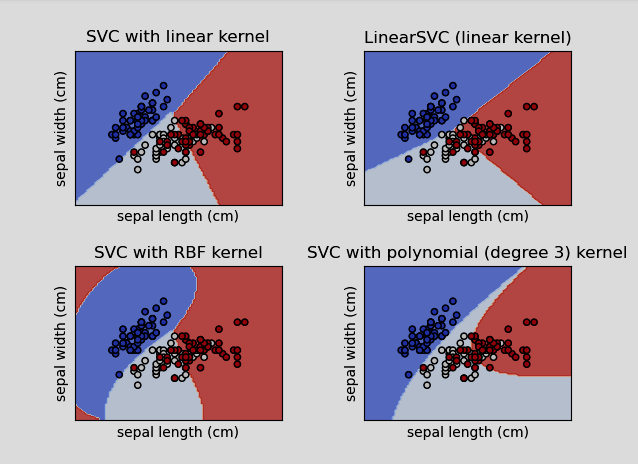
\includegraphics[width=0.75\linewidth]{kernel_types.png} % insira o caminho da sua imagem e ajuste a largura
      \caption{Superfície de separação de diferentes kernels na base de dados Iris.} % insira a legenda desejada
      \label{fig:exemplo} % rótulo para referenciar a figura no texto
   \end{figure}

   \vspace{1cm}

   Após um estudo mais aprofundado na escolha dos kernels, chega-se a seguinte conclusão : 

   \begin{enumerate}
      \item \textbf{Kernel Linear} = Utilizado quando a base de dados é aproximadamente linearmente separável. É o kernel mais simples e computacionalmente eficiente, pois não transforma os dados para um espaço dimensional mais alto. Ele é geralmente mais rápido e menos custoso em termos computacionais que os demais kernels, sendo ideal para grandes conjuntos de dados com características lineares.

      \item \textbf{Kernel Polinomial} = Adequado para conjuntos de dados com relações polinomiais entre características. Este kernel permite o ajuste de padrões complexos, sendo computacionalmente mais custoso, especialmente para polinômios de alto grau. O aumento do grau polinomial eleva a complexidade computacional e pode levar a problemas de sobreajuste (overfitting) se não for regulado adequadamente.

      \item \textbf{Kernel RBF (Radial Basis Function)} = Muito utilizado para características não lineares e uma das escolhas mais comuns no aprendizado de máquina. O kernel RBF projeta os dados para um espaço dimensional mais alto, permitindo uma separação não linear, o que o torna eficaz para dados complexos. Seu parâmetro \(\gamma\) controla a amplitude do kernel e deve ser cuidadosamente ajustado para evitar sobreajuste ou subajuste.

      \item \textbf{Kernel Sigmoidal} = Embora não seja um kernel amplamente utilizado em SVMs, é popular como função de ativação em redes neurais devido à sua capacidade de modelar relações não lineares. Em SVMs, o kernel sigmoidal é menos comum porque pode resultar em margens de separação menos estáveis, especialmente em dados de alta dimensionalidade.

   \end{enumerate}

   Como confirmação, foi testada uma SVM com um kernel sigmoidal, o qual se espera ter um baixo desempenho. Abaixo está registrada a matriz de confusão, confirmando a afirmação acima.

   \begin{figure}[h] % 'h' posiciona a figura aproximadamente no local do código
       \centering % centraliza a figura
       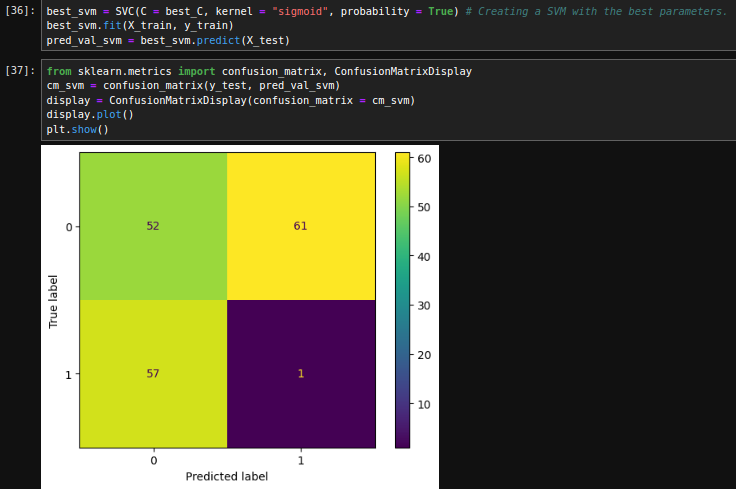
\includegraphics[width=0.75\linewidth]{sigmoidal_kernel.png} % insira o caminho da sua imagem e ajuste a largura
       \caption{Matriz de confusão usando um kernel sigmoidal.} % insira a legenda desejada
       \label{fig:exemplo} % rótulo para referenciar a figura no texto
   \end{figure}
   
   \vspace{1cm}
   
   Outro kernel testado foi o kernel polinomial, variando o seu grau. Como esperado, para um grau menor o desempenho foi melhor pois a base de dados é aproximadamente linearmente separável. Ao aumentar o valor do grau p, o tempo de execução aumentou consideravalemte, em conjunto com o overfitting. Ou seja, o modelo ficou muito complexo e se sobreajustou aos dados. As imagens abaixo mostram como o modelo teve um pior desempenho ao aumentar consideravalemte o valor de p, além de consumir mais recurso computacional.
   
   \vspace{1cm}
   \begin{figure}[htbp] % Use 'htbp' para melhor flexibilidade de posicionamento
      \centering % Centraliza a figura
  
      % Primeira subfigura
      \begin{subfigure}{0.75\textwidth} % Largura da primeira subfigura
          \centering
          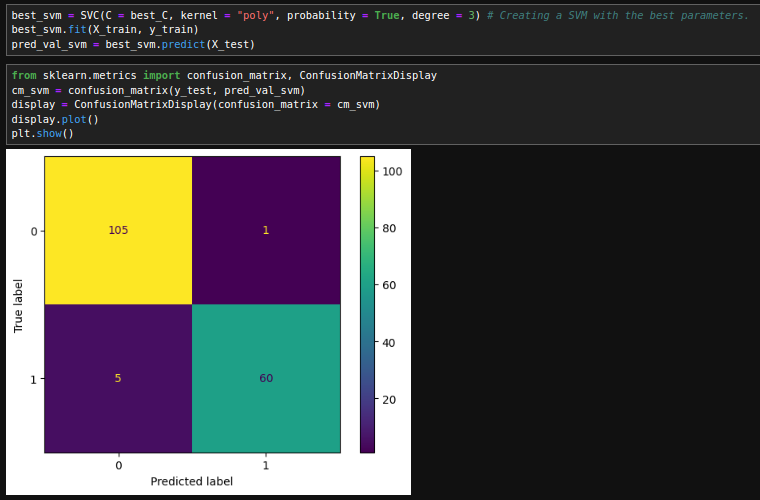
\includegraphics[width=\linewidth]{grau3.png} % Caminho para a imagem
          \caption{Matriz de confusão usando um kernel polinomial de grau 3.} % Legenda da primeira imagem
          \label{fig:exemplo2} % Rótulo único para a primeira imagem
      \end{subfigure}
      
      \vspace{0.5cm} % Espaço vertical entre as subfiguras
  
      % Segunda subfigura
      \begin{subfigure}{0.75\textwidth} % Largura da segunda subfigura
          \centering
          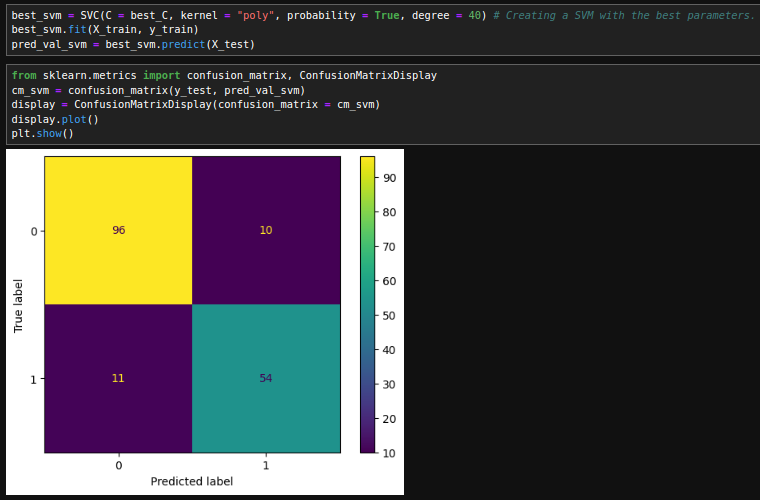
\includegraphics[width=\linewidth]{grau40.png} % Caminho para a imagem
          \caption{Matriz de confusão usando um kernel polinomial de grau 40.} % Legenda da segunda imagem
          \label{fig:exemplo3} % Rótulo único para a segunda imagem
      \end{subfigure}
  
      \caption{Comparação das matrizes de confusão para diferentes graus de kernel polinomial.} % Legenda geral para a figura
      \label{fig:matrizes_confusao} % Rótulo para a figura inteira
  \end{figure}

   \newpage

   Por fim, ao utilizar o kernel RBF e variar o parâmetro \(\gamma\), observa-se que valores altos de \(\gamma\) causaram overfitting no modelo; valores intermediários de \(\gamma\) permitiram uma boa generalização; e valores muito baixos resultaram em um desempenho ruim devido ao underfitting. As imagens abaixo ilustram as comparações em ordem crescente de \(\gamma\): 

   \begin{figure}[H] % Use [h] if you prefer flexibility in placement
      \centering % Center the entire figure
      
      \begin{subfigure}{0.75\textwidth} % Specify width for first subfigure
         \centering % Center the subfigure
         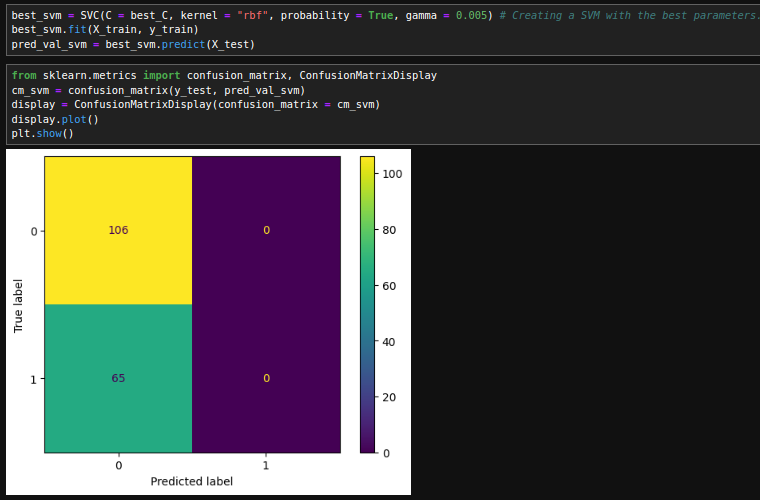
\includegraphics[width=\linewidth]{gamma0_5.png} % Path to your image
         \caption{Matriz de confusão usando um kernel RBF com \(\gamma\) = 0,5.} % Caption for the first image
         \label{fig:exemplo1} % Unique label for the first image
   \end{subfigure}
      \hfill % Horizontal space between subfigures
      
      \begin{subfigure}{0.75\textwidth} % Specify width for second subfigure
         \centering % Center the subfigure
         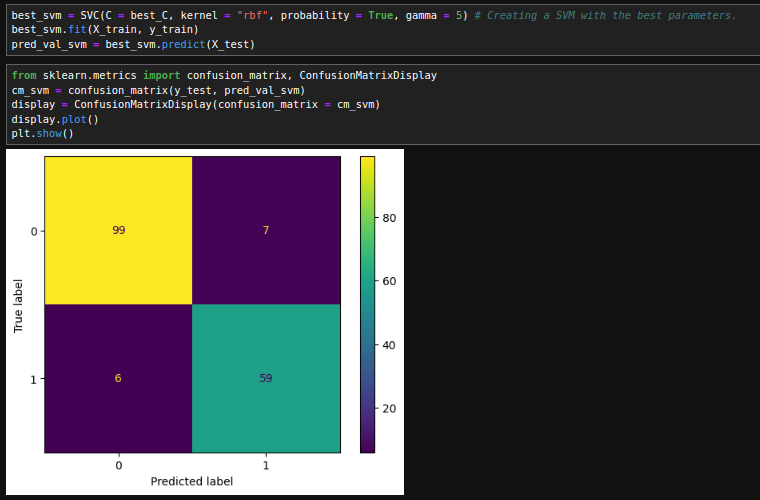
\includegraphics[width=\linewidth]{gamma5.png} % Path to your image
         \caption{Matriz de confusão usando um kernel RBF com \(\gamma\) = 5.} % Caption for the second image
         \label{fig:exemplo2} % Unique label for the second image
   \end{subfigure}
      \hfill % Horizontal space between subfigures
      \begin{subfigure}{0.75\textwidth} % Specify width for the third subfigure
         \centering % Center the subfigure
         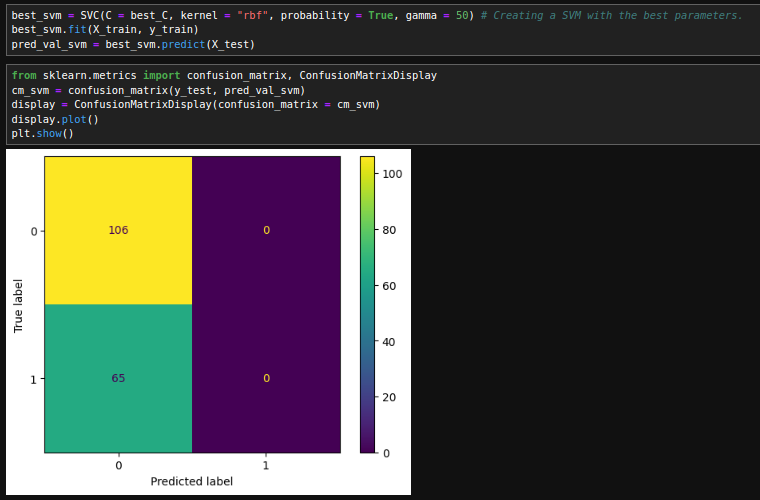
\includegraphics[width=\linewidth]{gamma50.png} % Path to your image
         \caption{Matriz de confusão usando um kernel RBF com \(\gamma\) = 50.} % Caption for the third image
         \label{fig:exemplo3} % Unique label for the third image
      \end{subfigure}

      \caption{Kernel RBF ao varias \(\gamma\).} % General caption for the figure
      \label{fig:imagens} % Label for the entire figure
   \end{figure}

   Para valores baixos de \(\gamma\), o modelo tende a dar pouca importância para a relação entre as amostras, resultando em um underfitting. Para um valor alto de \(\gamma\) o modelo dará muita importância para as amostras individuais, resultando em um overfitting. O ideal é encontrar um meio termo entre esses pontos de forma a não ter um overfitting nem um underfitting.

   \subsection{KNN}

   \vspace{1cm}

   Para o KNN ponderado, o melhor valor de K encontrado para a base de dados através do algoritmo GridSearch foi K = 2. Ao variar o hiperparâmetro h do KNN, variamos também a influência de cada amostra em relação ao novo ponto. Para valores baixos de h, o modelo resultou em um overfitting, pois as amostras mais próximas do ponto foram as únicas que tiveram influência no preditor. Enquanto um valor alto de h acrescentou custo computacional ao modelo, pois a abertura da gaussiana irá cobrir todos os pontos com um valor limiar de h. Ao passar desse valor de h, todos os pontos já serão cobertos pela mesma. A acurácia do modelo foi de apenas 78\%, consideravelmente inferior em relação a acurácia da SVM.


   \section{Conclusão}

   Portanto, ao aplicar os algoritmos de Machine Learning SVM e KNN ponderado na base de dados Breast Cancer, concluímos que o SVM apresentou o melhor desempenho. O kernel linear destacou-se em comparação com os demais kernels, sugerindo que a base de dados tende a ser linearmente separável. Os melhores hiperparâmetros para cada modelo foram obtidos por meio do algoritmo GridSearch. No caso da SVM, o hiperparâmetro C controlou a margem do modelo, definindo o equilíbrio entre viés (erro médio nos dados de treino) e variância (erro médio nos dados de teste). Um valor alto de C resulta em uma "hard-margin," que minimiza as amostras classificadas incorretamente, enquanto um valor baixo de C leva a uma "soft-margin," permitindo mais classificações incorretas para acomodar a generalização do modelo. O tipo de kernel mais adequado depende exclusivamente do conjunto de dados utilizado. Para o KNN, o hiperparâmetro K também influencia esse equilíbrio: valores baixos de K tendem a gerar overfitting, enquanto valores altos podem resultar em underfitting. A abertura da Gaussiana no KNN, determinada pelo valor de h, controla a influência dos K vizinhos mais próximos, sendo que valores baixos de h aumentam o risco de overfitting.
   
   \section{Referências utilizadas e o código}

   https://edition.cnn.com/2023/08/01/health/ai-breast-cancer-detection/index.html
   Código : https://github.com/arthurfreisouza/IRP-codes.
   % Results content here.

   \end{document}